\documentclass{article}
\usepackage[utf8]{inputenc}
\usepackage{amsthm}
\usepackage{amsmath}
\usepackage{amssymb}
\usepackage{enumitem}
\setlength{\parindent}{0em}
\setlength{\parskip}{1em}
\usepackage{fixltx2e}
\usepackage{graphicx}
\usepackage{float}
\newcommand{\Mod}[1]{\ (\mathrm{mod}\ #1)}
\usepackage{mathabx}
\usepackage{siunitx}
% \DeclareMathOperator{\tr}{tr}
\usepackage{geometry}
 \geometry{
 a4paper,
 total={170mm,257mm},
 left=20mm,
 top=20mm,
 }
\usepackage{mathtools} 
% \DeclarePairedDelimiter\abs{\lvert}{\rvert}
% \DeclarePairedDelimiter\norm{\lVert}{\rVert}

\newenvironment{QandA}{\begin{enumerate}[label=\bfseries\alph*.]\bfseries}
                      {\end{enumerate}}
\newenvironment{answered}{\par\normalfont}{}

\title{Calculus 19/20 Sem 1 Suggested Answers}

\author{\makebox[.9\textwidth]{NUS LaTeXify Proj Team}}
\date{Updated: 28 December 2019}

\begin{document}

\maketitle

Done by: Yip Jung Hon and Pan Jing Bin
\hline

\subsubsection*{Question 1}
\begin{enumerate}[label=\alph*)]
    \item True. First note that $f(x)$ is continuous on $(0,\pi/2)$. Then $f'(x) = 1 + \frac{\cos x}{\sin x}=1+\cot x$. On $(0,\pi/2)$, $\cot x > 0 \implies f'(x) > 0$. Thus, on $(0,\pi/2), f$ is continuous and strictly increasing and so $f$ has an inverse.
    \item False. Consider $f(x) = x^3$. Then $f'(x) = 3x^2.$ $f$ is an increasing function, but $f'(0) = 0$. Thus the statement is false.
    \item False.  Consider $f(x) = x^4$. Then $f'(x) = 4x^3$ and $f''(x) = 12x^2$. Note that $f$ has a local minimum at $x = 0$ but $f''(0) = 0$ thus the statement is false.
    \item False. $f$ can be a strictly increasing function, in which case $f'(c) \neq 0 \  \forall x\in (0,1)$.
    \item True. First note that since $f$ is continuous on $[-1,1]$, $f(x)$ is defined $\forall x\in [-1,1]$. Thus $\int^1_{0} f(x) dx$ and $\int^0_{-1} f(x) dx$ exists.
    
    Since $f$ is odd, then $f(x) = -f(-x)$. Then one has:
    \begin{align*}
        \int^1_{-1} f(x) dx&=\int^1_{0} f(x) dx +\int^0_{-1} f(x) dx \\
        &= \int^1_{0} f(x) dx +\int^0_{-1}-f(-x)dx \\
        &= \int^1_{0} f(x) dx +\int^0_{1}f(u)du \ \ \text{(Sub $u = -x$, $\frac{du}{dx}=-1$)} \\
        &= \int^1_{0} f(x) dx -\int^1_{0}f(u)du\\
        &= 0
    \end{align*}
\end{enumerate}

\pagebreak
\subsubsection*{Question 2}
\begin{enumerate}[label=\alph*)]
    \item $\sin(x^2+1)+2x^2\cos(x^2+1)$
    \item $D=\int^{\pi/2}_0 |\cos(2t)| dt = 1$. 
    \item $\int_0^1 f(x) dx \approx 0.25 \times 1 + 0.25 \times 0 +0.25 \times 2 + 0.25 \times 0 = 0.75$.
    \item $f(0.0001) \approx f(0) + 0.0001f'(0) = 1.0002$.
    \item $e^{2a}\tan(a)$
    \begin{align*}
        \int_0^a e^{2x}(\tanx+1)^2 \ dx &= \int_0^a e^{2x}\tan^2x \ dx + \int_0^a e^{2x}2\tan x \ dx + \int_0^a e^{2x} \ dx \\
        &= \int_0^a e^{2x}\sec^2x \ dx + \int_0^a 2e^{2x}\tan x \ dx \\
        &= \int_0^a e^{2x}\sec^2x \ dx + e^{2x}\tan x\Big|^{a}_0 - \int_0^a e^{2x}\sec^2x \ dx \ \ \text{(By IBP on $ 2e^{2x}\tan x$)} \\
        &= e^{2a}\tan(a)
    \end{align*}
\end{enumerate}

\subsubsection*{Question 3}
\begin{enumerate}[label=\roman*)]
    \item Define $h(x) = f(x) - g(x)$. Then $h(x) = -3x^2 - 12x + 1 - x^3/3 - \sin(2x)$.
    
    $h(0) = 1, h(1) = -\frac{43}{3} - \sin(2)< 0$.

    Since $h(0) = 1 > 0$ and $h(1) < 0$ and $h$ is continuous on $\mathbb{R}$ , by IVT, $ \exists \ c \in (0,1)$ such that $h(c) = 0 \implies f(c) = g(c)$.
    
    \item We first suppose there 2 roots. Assume that $\exists \ c_1,c_2 \in \mathbb{R}$ such that $h(c_1) = h(c_2) = 0$. WLOG, let. $c_2 > c_1$.
    \begin{align*}
        h'(x) &= -6x - 12 - x^2 - 2\cos(2x) \\
        &= -(x+3)^2 - 2\cos(2x) - 3
    \end{align*}
    Note that $-(x+3)^2\leq 0$ and $-2\cos(2x) - 3 < 0$. Thus $h'(x) < 0 \ \forall x \in \mathbb{R}$.
    
    Since $h$ is continuous and differentiable on $\mathbb{R}$, by the MVT, $\exists d \in (c_1,c_2)$ such that $h'(d) = 0$. This is a contradiction as we have just shown $h'(x) < 0$.
\end{enumerate}

\pagebreak
\subsubsection*{Question 4}
$f(x)=(x-6)^{2/3}(5-x)^{2/3}$.
\begin{flalign}
    f'(x)=\frac{16-3x}{3(x-6)^{1/3}(5-x)^{2/3}}&&
\end{flalign}
Note that $(5-x)^{2/3}$ is always positive. 
\begin{enumerate}[label=(\roman*)]
    \item When $f'(x) > 0$, you need $16-3x>0 \ \text{and} \  x-6>0 \implies x<16/3 \ \text{and} \  x>6$. You could also have $16-3x<0 \ \text{and} \  x-6<0 \implies x>16/3 \ \text{and} \  x<6$.
    
    For $f'(x) < 0$, you need $16-3x<0 \ \text{and} \  x-6>0 \implies x>16/3 \ \text{and} \  x>6$. You could also have $16-3x>0 \ \text{and} \  x-6<0 \implies x<16/3 \ \text{and} \  x<6$. 
    
    We also have to check $f'(x)$ at the points near where $f'(x)$ is undefined:
    \begin{center}
         \begin{tabular}{||c c c c c||} 
         \hline
         $x$ & 5^- & 5^+ & 6^- & 6^+ \\
         \hline\hline
         $f'(x)$ & -ve & -ve & +ve & -ve \\ 
         \hline
        \end{tabular}
    \end{center}
    Thus, we have that $f(x)$ is increasing on the open interval $(16/3, 6)$ and $f(x)$ is decreasing on the open interval $(-\infty, 16/3)$ and $(6, \infty)$. 
    
    \item When $f'(x)=0, x=16/3$. 
        \begin{center}
         \begin{tabular}{||c c c||} 
         \hline
         $x$ & 16/3^- & 16/3^+ \\
         \hline\hline
         $f'(x)$ & -ve & +ve \\ 
         \hline
        \end{tabular}
    \end{center}
    From the table in part (i), we also note that 6 is a local maximum point. We have:
    
    Local min: $(16/3, -\frac{1}{3}(2^{2/3}))$ \\
    Local max: $(6,0)$
\end{enumerate}

\pagebreak
\subsubsection*{Question 5}
\begin{enumerate}[label=\alph*)]
\item Let $\epsilon > 0$. Choose $\delta = \min\{\epsilon/7,1\}$. Then whenever $0<|x-1|<\delta$,
\begin{align*}
    \left|\frac{1}{x^3+1} - \frac{1}{2}\right| &= 
    \left|\frac{2-x^3-1}{x^3+1}\right|\\
    &= \left|\frac{1-x^3}{x^3+1}\right|\\
    &= \left|\frac{x^3-1}{x^3+1}\right|\\
    &= \left|\frac{(x-1)(x^2+x+1)}{x^3+1}\right|\\
    &= \left|\frac{(x-1)[(x-1)^2+3(x-1)+3]}{x^3+1}\right|\\
    &\leq \left|\frac{|x-1|(|x-1|^2+3|x-1|+3)}{x^3+1}\right|\\
    &< \frac{\delta(\delta^2 + 3\delta + 3)}{1}\\
    & \leq 7\delta\\
    & \leq \epsilon
\end{align*}

\item Define $f(t) =\sqrt{t^2+t+1}-\sqrt{t^2-t}$ \\
\begin{align*}
    \lim_{x\to\infty}\frac{\int^x_{1}(\sqrt{t^2+t+1}-\sqrt{t^2-t})(x-t)dt}{x^2+x+1}&=\lim_{x\to\infty}\frac{x\int^x_{1}f(t)dt-\int^x_{1}tf(t)dt}{x^2+x+1}\\
    \intertext{Since the top and bottom goes to infinity, we can apply L'Hopital's Rule. The term $x\int^x_{1}f(t)dt$ can be differenciated using the product rule.}
    &=\lim_{x\to\infty} \frac{xf(x)+\int^x_{1}f(t)dt-xf(x)}{2x+1} \\
    &=\lim_{x\to\infty} \frac{\int^x_{1}f(t)dt}{2x+1}\\
    \intertext{The top and bottom goes to infinity, and we apply L'Hopital's Rule again.}
    &=\lim_{x\to\infty} \frac{f(x)}{2} \\
    &=\lim_{x\to\infty}\frac{\sqrt{x^2+x+1}-\sqrt{x^2-x}}{2}\\
    \intertext{The trick to evaluating these kinds of limits is to rationalise the surd and mutiply $1/x$ to both the top and bottom.}
    &=\lim_{x\to\infty}\frac{\sqrt{x^2+x+1}-\sqrt{x^2-x}}{2} . \frac{\sqrt{x^2+x+1}+\sqrt{x^2+x}}{\sqrt{x^2+x+1}+\sqrt{x^2+x}} \\
    &=\lim_{x\to\infty}\frac{2x+1}{2\left[\sqrt{x^2+x+1}+\sqrt{x^2-x}\right]}\\
    &=\lim_{x\to\infty}\frac{2+1/x}{2\left[\sqrt{1+1/x+1/x^2}+\sqrt{1-1/x}\right]}\\
    &=\frac{2}{2(1+1)}=\frac{1}{2}
\end{align*}
\end{enumerate}

\pagebreak
\subsubsection*{Question 6}
\begin{enumerate}[label=\alph*)]
    \item We first implicitly differenciate the curve. We obtain:
    \begin{align*}
        &\frac{2}{3}x^{-1/3}+\frac{2}{3}\frac{dy}{dx}y^{-1/3}=0 \\ 
        &x^{-1/3}+\frac{dy}{dx}y^{-1/3}=0 \\
        &\frac{dy}{dx}=-\frac{-y^{1/3}}{x^{1/3}} 
    \intertext{So one has:}
        &1+(\frac{dy}{dx})^2=\frac{y^{2/3}}{x^{2/3}} + \frac{x^{2/3}}{x^{2/3}}=\frac{1}{x^{2/3}}
    \intertext{We first calculate the length of the curve, $L$, for just the first quadrant.}
        \frac{1}{4}L&=\int^1_0 \sqrt{1+f'(x)} \ dx \\ &=\int^1_0\sqrt{\frac{1}{x^{2/3}}} \ dx \\
        &=\int^1_0 \frac{1}{x^{1/3}} \ dx \\
        &=\frac{3}{2}x^{2/3}\Big|^1_0 \\
        &=\frac{3}{2}
    \end{align*}
    So $L=6$.
    
    \item Using $\text{Surface Area} &= \int 2\pi f(x) \sqrt{1+f'(x)} \ dx$.
    \begin{align*}
        \text{Surface Area} &= \int^{\pi/2}_{-\pi/2} 2\pi \cos x \sqrt{1+\sin^2x } \ dx
    \intertext{Let $u=\sin x, du/dx=\cos x $,}
        &= \int^{1}_{-1} 2\pi \cos x \sqrt{1+u^2 } \ \frac{du}{\cos x } \\
        &= \int^{1}_{-1} 2\pi \sqrt{1+u^2 } \ du \\
    \intertext{Let $u=\tan x, du/dx=\sec^2 x$.} 
        &= \int^{\pi/4}_{-\pi/4} 2\pi \sec x \sec^2 x \ dx \\
        &= 2\pi \int^{\pi/4}_{-\pi/4} \sec^3 x \ dx \\
        &=2\pi \left  [\frac{1}{2}\sec\left(\frac{\pi}{4}\right)\tan\left(\frac{\pi}{4}\right)+\frac{1}{2}\ln\left(\sec\left(\frac{\pi}{4}\right)+\tan\left(\frac{\pi}{4}\right)\right)\right]-\\
        & \ \ \ \ 2\pi \left[ \frac{1}{2}\sec\left(-\frac{\pi}{4}\right)\tan\left(-\frac{\pi}{4}\right)+\frac{1}{2}\ln\left(\sec\left(-\frac{\pi}{4}\right)+\tan\left(-\frac{\pi}{4}\right) \right)\right] \\
        &=\pi \left[ \sqrt{2} + \ln(\sqrt{2}+1) - ( \sqrt{2} +\ln(\sqrt{2}-1) \right] \\
        &=\pi \left[2\sqrt{2}+\ln\frac{\sqrt{2}+1}{\sqrt{2}-1} \right]
    \end{align*}
    
\pagebreak
    
\item Note that this is equivalent to finding the volume of $y=e^{x-1}$ revolving about $x=0$ from $x=1$ to $x=2$.

\begin{figure}[H]
    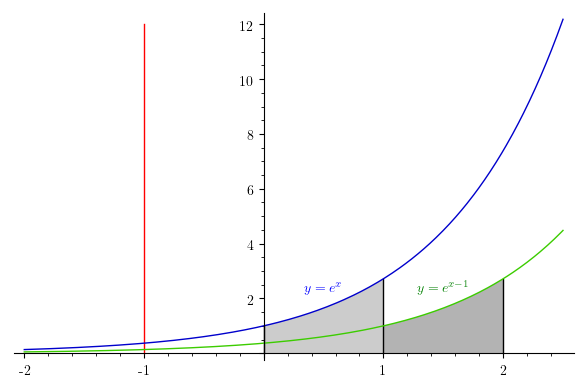
\includegraphics[width=16cm]{qn6c.png}
    \centering
\end{figure}

By method of cylindrical shells,
\begin{align*}
    \text{Volume} &= \int^2_1 2\pi xe^{x-1} \ dx
\intertext{Let $u=x-1$,}
    &= \int^1_0 2\pi (u+1)e^u \ du \\
    &= 2\pi \left[\int^1_0 ue^u \ du +  \int^1_0 e^u \ du\right]\\
    &= 2\pi \left[ue^u\Big|^1_0 - \int^1_0 e^u \ du + \int^1_0 e^u \ du \right] \ \ \text{(By IBP on $ue^u$)}\\ 
    &= 2\pi e
\end{align*}
    
\end{enumerate}

\pagebreak
\subsubsection*{Question 7}
\begin{enumerate}[label=\alph*)]
\item This is a homogeneous DE.
\begin{align*}
    \frac{dy}{dx}&=\frac{x^2-y^2}{2xy}=\frac{1}{2}\left(\frac{x}{y}\right)-\frac{1}{2}\left(\frac{y}{x}\right) \\
    \intertext{Substitute $z=y/x$, then $\frac{dy}{dx}=z+x\frac{dz}{dx}$.}
    &\frac{dz}{dx}x+z=\frac{1}{2z}-\frac{1}{2}z\\
    &\frac{dz}{dx}x=\frac{1}{2}\left(\frac{1-3z^2}{z}\right)\\
    &\frac{z}{1-3z^2}\frac{dz}{dx}=\frac{1}{2x}\\
    &\int\frac{z}{1-3z^2}dz=\frac{1}{2}\int\frac{1}{x}dx\\
    &-\frac{1}{3}\ln|1-3z^2|=\ln{x} + C \ \ \text{($x>0$)}\\
    &\ln\left|1-3\left(\frac{y}{x}\right)^2\right|=-3\ln{x} -3C \\
    &\left|1-3\left(\frac{y}{x}\right)^2\right| = e^{-3\ln{x}-3C}\\
    &1-3(\frac{y}{x})^2= Ae^{-3\ln{x}} \ \ \text{(A=$\pm e^{-3C}$)}\\
    &1-3\left(\frac{y}{x}\right)^2=\frac{A}{x^3}\\
    &3\left(\frac{y}{x}\right)^2=1-\frac{A}{x^3}\\
    &y^2 = \frac{1}{3}x^2-\frac{A}{3x}\\
\intertext{When $x=1,y=1, A=-2$.}
    &y^2=\frac{1}{3}x^2+\frac{2}{3x}\\
    &y=\pm \sqrt{\frac{1}{3}x^2+\frac{2}{3x}}\\
    &y=\sqrt{\frac{1}{3}x^2+\frac{2}{3x}} \ \ \text{(Rej -ve, $y>0$)}
\end{align*}

\item Let $x$ be the fertiliser in the tank at time $t$. Let V be the volume of water in the tank at time $t$.

Rate of adding fertiliser = $0.1*4 = 0.4$.

Rate of fertiliser pumped out $=12x/V$.

Note that $V = 400-8t$.
\begin{align*}
    &\frac{dx}{dt} = 0.4 - \frac{12x}{400-8t}\\
    &\frac{dx}{dt}+\frac{12x}{400-8t}=0.4\\
\intertext{Find integrating factor:}
    e^{\int\frac{12}{400-8t}dt}&= e^{-\frac{3}{2}\ln{|400-8t|}}\\
    &=(400-8t)^{-\frac{3}{2}} \ \ \text{(Note that $400-8t\geq 0$)}.
\intertext{Mutiplying $(400-8t)^{-\frac{3}{2}}$ to both sides and integrating, we get:}
    (400-8t)^{-\frac{3}{2}}x&=\int{0.4(400-8t)^{-\frac{3}{2}}}dt\\
    &=\frac{1}{10}(400-8t)^{-\frac{1}{2}}+C \\
    x&=\frac{1}{10}(400-8t)+C(400-8t)^\frac{3}{2}.
\intertext{When $t=0,x=0$.}
    &0=40+C(400)^\frac{3}{2} \implies C=-\frac{1}{200}\\.
\intertext{So one has that,}
    &x=40-\frac{4}{5}t - \frac{(400-8t)^\frac{3}{2}}{200}
\intertext{At maximum fertiliser, $\frac{dx}{dt}=0$.}
    &0.4=\frac{12x}{400-8t}\\
    &x=\frac{400-8t}{30}\\
    &\frac{400-8t}{30}=40-\frac{4}{5}t-\frac{(400-8t)^\frac{3}{2}}{200}\\
    &(400-8t)^\frac{3}{2}=\frac{40}{3}(400-8t)\\
\intertext{Moving all the terms to one side and factorising,}
    &400-8t=0 \  \text{or} \  (400-8t)^\frac{1}{2} = \frac{40}{3}\\
    &t=50 \ \text{or} \  400-8t = \frac{1600}{9}\\
    &t = \frac{250}{9}
\end{align*}
Note that when $t\geq50,x=0$ as all the water has been drained away.

At $t=250/9,x=160/27$.

Thus the maximum amount of fertiliser in the tank is $x=160/27$ and the time required to reach it is $t=250/9$.

\end{enumerate}

\pagebreak
\textbf{Question 8}

Note the following identities:
\begin{equation*}
    \sin^2(x/2)=\frac{1-\cos x}{2} \ \ \ \cos^2(x/2)=\frac{1+\cos x}{2}
\end{equation*}
Also note that $1+a\cos x=A(1+\cos x)+B(1-\cos x)$ where $A+B=1, A-B=a$.

Solving, we have $A=\frac{1}{2}(1+a), B=\frac{1}{2}(1-a)$.

So we can write:
\begin{align*}
    \frac{1}{1+a\cos x}&=\frac{1}{\frac12(1+a)(1+\cos x)+\frac12(1-a)(1-\cos x)}\\
    &=\frac{1}{(1+a)\cos^2(x/2)+(1-a)\sin^2(x/2)}  \\
    &=\frac{1}{1+a}\frac{\sec^2(x/2)}{1+\frac{1-a}{1+a}\tan^2(x/2)}\\
\intertext{If $a=1$, then we have:}
    &\int \frac{1}{1+a} \sec^2{(x/2)}\ dx=\int \frac{1}{2} \sec^2{(x/2)}\ dx =\tan{(x/2)}+c
\intertext{If $a<1$, sub $t=\sqrt{\frac{1-a}{1+a}}\tan(x/2)$, then $\frac{dx}{dt}=\sqrt{\frac{1+a}{1-a}}\frac{2}{\sec^2{(x/2)}}$.}
    \int \frac{1}{1+a}\frac{\sec^2(x/2)}{1+\frac{1-a}{1+a}\tan^2(x/2)} \ dx&= \int \frac{1}{1+a}\frac{\sec^2(x/2)}{1+t^2}\sqrt{\frac{1+a}{1-a}}\frac{2}{\sec^2{(x/2)}}\ dt \\
    &= \int \frac{1}{\sqrt{(1+a)(1-a)}}\frac{2}{1+t^2} \ dt \\
    &= \int \frac{1}{\sqrt{1-a^2}}\frac{2}{1+t^2} \ dt \\
    &= \frac{2\tan^{-1}{t}}{\sqrt{1-a^2}}+c \\
    &= \frac{2\tan^{-1}\left[{\sqrt{\frac{1-a}{1+a}}\tan(\frac{x}{2})}\right]}{\sqrt{1-a^2}}+c
\intertext{Else, if $a>1$, sub $t=\sqrt{\frac{a-1}{1+a}}\tan(x/2)$, then
$\frac{dx}{dt}=\sqrt{\frac{1+a}{a-1}}\frac{2}{\sec^2{(x/2)}}$.}
    \int \frac{1}{1+a}\frac{\sec^2(x/2)}{1+\frac{1-a}{1+a}\tan^2(x/2)} \ dx&= \int \frac{1}{1+a}\frac{\sec^2(x/2)}{1-t^2}\sqrt{\frac{1+a}{a-1}}\frac{2}{\sec^2{(x/2)}}\ dt \\
    &= \int \frac{1}{\sqrt{(1+a)(a-1)}}\frac{2}{1-t^2} \ dt \\
    &= \int \frac{1}{\sqrt{a^2-1}}\frac{2}{1-t^2} \ dt \\
    &= \frac{1}{\sqrt{a^2-1}}\ln \left|{\frac{t+1}{t-1}} \right|+ c \\
    &= \frac{1}{\sqrt{a^2-1}}\ln \left|{{\frac{\sqrt{\frac{a-1}{1+a}}\tan(\frac{x}{2})+1}{\sqrt{\frac{a-1}{1+a}}\tan(\frac{x}{2})-1}}}\right|+ c
\end{align*}
\end{document}


